\section{Experimental Details} \label{app:exp_detail}
\subsection{Default Experimental Setup} \label{app:exp_default}

As many of our experiments share a similar setup, we begin by outlining the default configuration. Most implementation details and hyperparameters follow those of SiT~\citep{ma2024sit}.

\textbf{Dataset.}~We conduct all of our real-world image generation experiments on ImageNet at $256 \times 256$, consisting of $N = 1281167$ images across $1000$ classes. We apply horizontal flip augmentation during preprocessing, effectively doubling the dataset size to $|\train| = 2N$.

\textbf{Diffusion.}~We use simple linear interpolants with $\alpha_t = 1 - t$ and $\sigma_t = t$, and adopt the $\rvv$-prediction objective. The velocity $\rvv_\rvtheta$ is related to the score $\rvs_\rvtheta$ by the linear relation $\rvv_\rvtheta(\rvz_t, t) = -\frac{t}{1 - t}\rvs_\rvtheta(\rvz_t, t) - \frac{1}{1-t}\rvz_t$. As an exception, models in \Cref{exp:foe} uses $\rvx$-prediction for numerical stability, which is also linearly related to the score: $\rvx_\rvtheta (\rvz_t, t) = \frac{t^2}{1 - t}\rvs_\rvtheta(\rvz_t, t) + \frac{1}{1 - t}\rvz_t$.  For sampling, we use the \texttt{dopri5} adaptive ODE solver with \texttt{atol=1e-6} and \texttt{rtol=1e-3}.

\textbf{Training.}~Models are trained on 4 NVIDIA H100 GPUs with the AdamW optimizer~\citep{loshchilov2017decoupled} (no weight decay), with $(\beta_1, \beta_2) = (0.9, 0.999)$, a constant learning rate of $10^{-4}$, and batch size of $256$ for $400$K training iterations. We maintain an exponential moving average (EMA) of model weights with a decay rate of 0.9999. All models are latent diffusion models trained on $32\times32\times4$ latents precomputed using SD-VAE~\citep{rombach2022high}. Additionally, all models are \emph{class-conditional}, modeling 1000 distinct distributions, and trained with a class dropout probability of 0.1 to enable estimation of \emph{unconditional} scores. We employ two different architectures:
{\setlength{\parskip}{2pt}\begin{enumerate}[leftmargin=*,label=(\arabic*),nosep,itemsep=2pt]
    \item Diffusion Transformer: Following the SiT architecture~\citep{ma2024sit}, with four configurations (S, B, L, XL), using a patch size of 2.
    \item U-Net: Based on \citet{dhariwal2021diffusion}, with four configurations (XS, S, B, L) varying model channels~\citep{karras2024analyzing} as $(64, 128, 192, 320)$. Attention layers are applied at resolutions $(1, 2, 4)$, except in the convolution-only U-Net, where attention is disabled.
\end{enumerate}}

Unless otherwise specified, we primarily use diffusion transformers (SiT) in our experiments.

\textbf{Evaluation.}~For FID evaluation, we follow the protocol of \citet{dhariwal2021diffusion} using their official implementation. FLOPs are measured with \texttt{ptflops}~\citep{ptflops}, and total training compute is calculated as FLOPs per forward pass multiplied by the number of training iterations.

\textbf{Supervision and Extrapolation Regions.}~Many of our experiments measure the expectation of a given \emph{quantity $\gQ$}, $\E[\gQ]$, separately over the supervision and extrapolation regions. As these regions correspond to continuous probability distributions in the data space, we report Monte Carlo estimates by sampling from each region and averaging the computed quantities.

For the supervision region, we sample $\rvz_t^{\text{sup}}$ from $\hat{p}_t$ by randomly selecting a training data point $\rvx$ and Gaussian noise $\rvepsilon$, then running the forward process: $\rvz_t^\text{sup} = \alpha_t \rvx + \sigma_t \rvepsilon$, identical to the training procedure. For the extrapolation region, we sample $\rvz_t^\text{ext}$ from an inference trajectory, obtained by solving the ODE with a pretrained model starting from random noise $\rvz_1^\text{ext} = \rvepsilon$. We then average the quantity $\gQ$ over $N$ samples:
$$\hat{\E}_t^{\text{sup}} (\gQ) = \frac{1}{N}\sum_{i = 1}^{N} \gQ(\rvz_t^{i,\text{sup}}, t), \;\hat{\E}_t^{\text{ext}} (\gQ) = \frac{1}{N}\sum_{i = 1}^{N} \gQ(\rvz_t^{i,\text{ext}}, t).$$
Often, we measure $\gQ$ across all timesteps rather than per timestep. In these cases, we use a timestep-dependent weighting function $\lambda(t)$ to ensure comparable scales across timesteps. Specifically, we sample $T$ random timesteps $\{t_j\}_{j=1}^{N}$ from $\operatorname{Unif}(0, 1)$ and repeat the above process, yielding:
$$\hat{\E}^\text{sup}(\gQ, \lambda) = \frac{1}{NT}\sum_{i=1}^N\sum_{i=1}^T \lambda(t_j) \gQ(\rvz_{t_j}^{i,\text{sup}}, t_j),\;\hat{\E}^\text{ext}(\gQ, \lambda) = \frac{1}{NT}\sum_{i=1}^N\sum_{i=1}^T  \lambda(t_j) \gQ(\rvz_{t_j}^{i,\text{ext}}, t_j).$$

Here, $\{\rvz_{t_j}^{i,\text{sup}}\}_{j=1}^T$ vary only in timesteps for the same data-noise pair $(\rvx, \rvepsilon)$, and $\{\rvz_{t_j}^{i,\text{ext}}\}_{j=1}^T$ vary only in timestep along the same inference trajectory. For the rest of the appendix, we simply specify $N$ and $\gQ$ (and $T$ and $\lambda$, if integrating over all timesteps), using the above notations.

\subsection{Details on CFG Paradox Experiment (\Cref{example:cfg})} \label{app:exp_cfg}

In \Cref{example:cfg}, we plot the difference between conditional and unconditional scores, $\|\rvs^c - \rvs^\varnothing\|$, in both the supervision and extrapolation regions. The difference is measured separately at $100$ different timesteps, $t = \{0.01, 0.02, \dots, 1.00\}$, using $\hat{\E}_t^{\text{sup}}(\gQ)$ and $\hat{\E}_t^{\text{exp}}(\gQ)$ of \Cref{app:exp_default} as described in \Cref{app:exp_default}. For the supervision region, we use $\gQ (\rvz_t, t) = \|\rvs_\star^c (\rvz_t, t) - \rvs_\star^\varnothing (\rvz_t, t)\|$ (difference of the empirical score), and for the extrapolation region, $\gQ (\rvz_t, t) = \|\rvs_\rvtheta^c (\rvz_t, t) - \rvs_\rvtheta^\varnothing (\rvz_t, t)\|$ (difference of the learned score) for the extrapolation region, with $N = 200$ samples per timestep.  For better visualization, we plot the median (dashed line) and the $10–90\%$ percentile range (shaded area) for each timestep.


\subsection{Details on Extrapolation During Inference Experiment (\Cref{exp:geometry-inference})}

In \Cref{exp:geometry-inference}, we plot the $r_\star$ values defined in \Cref{eq:r_star} measured in the supervision and extrapolation regions (\Cref{fig:extrapolation-b}). Similarly to \Cref{app:exp_cfg}, we measure the $r_\star$ values on 100 different timesteps, with $N = 100$ samples per timestep. For clarity, we plot each training data point and each sampling trajectory as a separate line, rather than showing averages.

\subsection{Details on Memorization Experiment (\Cref{exp:memorization-training})}

In \Cref{exp:memorization-training}, we sample $N = 200$ images $\rvx^{(i)} \in \train$ from the training dataset. For each image, we construct a noisy image $\rvz_t = \alpha_t \rvx^{(i)} + \sigma_t \rvepsilon$ at 21 timesteps $t = {0.00, 0.05, 0.10, \dots, 1.00}$. We then run ODE sampling ($t \to 0$) from each noisy image $\rvz_t$ and compare the final output to the original image $\rvx^{(i)}$. \Cref{fig:phase-transition} (left) shows a qualitative example, while \Cref{fig:phase-transition} (right) plots the memorization ratio, defined as the fraction of sampled images for which the $\ell_2$-closest image in the training set is the original $\rvx^{(i)}$ (following the calibrated $\ell_2$ metric in~\citet{carlini2023extracting}). Additionally, the overlap coefficient from \Cref{app:theory_overlap} is measured on the class-conditional distribution for a single class (red panda, $\text{id}=387$).


\subsection{Details on Supervision vs.\ Extrapolation Experiment (\Cref{exp:contrastive-scaling})}

In \Cref{exp:contrastive-scaling}, we measure the score error $\|\rvs_\theta - \rvs_\star\|^2$ in the supervision and extrapolation regions across different model sizes. The score error in each region is computed as $\hat{\E}^\text{sup}(\gQ, \lambda)$ and $\hat{\E}^\text{ext}(\gQ, \lambda)$ described in \Cref{app:exp_default}, using the following parameters: $\gQ(\rvz_t, t) = \|\rvs_\rvtheta(\rvz_t, t) - \rvs_\star(\rvz_t, t)\|^2$, $\lambda(t) = \frac{t^2}{(1 - t)^2}$, $N = 1000$, and $T = 100$. The weighting function $\lambda(t)$ is chosen so that $\lambda(t) \gQ(\rvz_t, t) = \|\rv_\rvtheta(\rvz_t, t) - \rvv_\star(\rvz_t, t)\|^2$, which reflects the $\rvv$-prediction objective and ensures uniform aggregation of the score error across timesteps.

\newpage
\subsection{Verification of Selective Underfitting in Gaussian (\Cref{sec:selective})} \label{app:selective-gaussian}

In this section, we empirically show that selective underfitting persists even with a Gaussian distribution.

\textbf{Setup.}~We consider a synthetic setup where the ground truth data distribution is Gaussian: $p_{\text{data}}=\gN(0,\mI)$ in $d = 20$ dimensions, with ground truth score $\rvs_{\textbf{gt}}(\rvz_t,t):=-{\rvz_t}/{\sigma_t}$. We construct a finite training set $\train$ by randomly sampling $|\train| = 100$ data points from $p_{\text{data}}=\gN(0,\mI)$. We train an MLP (10 layers, width 1000) for 20,000 iterations using Adam~\citep{kingma2014adam} with learning rate $4\times10^{-3}$. Every 100 iterations, we evaluate the learned score $\rvs_\rvtheta$, the empirical score $\xxgreen{\rvs_\star}$, and the ground truth score $\xxpurple{\rvs_{\textbf{gt}}}$.

\begin{minipage}{0.63\textwidth}
\textbf{Result.}~\Cref{fig:selective-gaussian} visualizes $\|\rvs_\rvtheta - \xxgreen{\rvs_\star}\|^2$ and $\|\rvs_\rvtheta - \xxpurple{\rvs_\textbf{gt}}\|^2$ in the supervision region (integrated by $\hat{p}_t$), and $\|\rvs_\rvtheta - \xxpurple{\rvs_\textbf{gt}}\|^2$ in the entire data space (integrated by $p_{\text{data}}$). In the supervision region, the error between the learned score and the ground truth score plateaus (\coloredul{xblue}{solid blue}), while the learned score converges to the empirical score (\coloreddashul{xblue}{dashed blue}), indicating no underfitting. In contrast, outside of the supervision region, the model's learned score approaches the ground truth score (\coloreddashul{xred}{dashed red}), indicating underfitting. This verifies that selective underfitting persists even for a simple Gaussian.
\end{minipage}
\hfill
\begin{minipage}{0.35\textwidth}
    \begin{figure}[H]
    \centering
    \vskip -1.5\baselineskip
    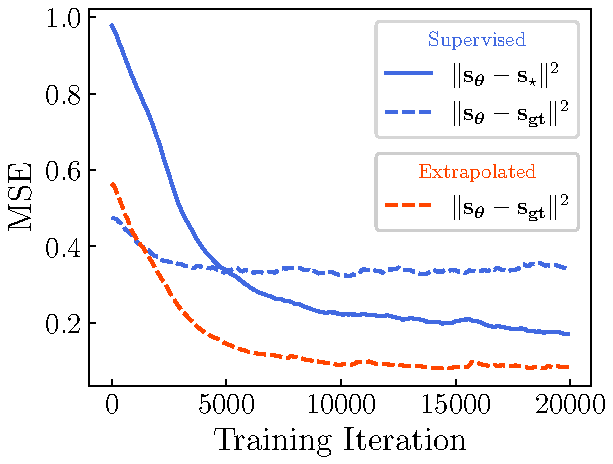
\includegraphics[width=\textwidth]{figures/generalization/selective_gaussian}
    \vskip -0.75\baselineskip
    \caption{\textbf{Gaussian Verification}.}
    \label{fig:selective-gaussian}
\end{figure}
\end{minipage}

\subsection{Details on Freedom of Extrapolation experiment (\Cref{exp:foe})} \label{app:exp_foe}

We detail the setup of the \emph{freedom of extrapolation} experiment, including subset construction, training procedure, and evaluation metric.

\textbf{Score and Region Subsets.}~As described in \Cref{sec:freedom}, we use two nested subsets $\trainsp \subseteq \trainrp$, drawn from the ImageNet training set $\train$. These subsets play distinct roles in the DSM objective:
$\trainsp$ defines the target (empirical) score $\rvs_\star$, while $\trainrp$ defines the data distribution $\hat{p}_t$ for sampling inputs in the DSM objective:
\begin{equation} \label{eq:appendix_dsm}
\Ls_{\text{DSM}} (t) = \E_{\xblue{\rvz_t \sim \hat{p}_t}} \left\|\rvs_\rvtheta (\rvz_t, t) - \xxgreen{\rvs_\star (\rvz_t, t)}\right\|^2.
\end{equation}
To construct $\trainsp$, we sample $100$ images per ImageNet class, resulting in $\trainsabsp = 1000 * 100 = 10^5$ images. To obtain $\trainrp$ of varying sizes while preserving $\trainsp$, we augment $\trainsp$ with additional images sampled uniformly without replacement from the remaining images in each class. Fixing $\trainsp$ and varying $\trainrp$, we train both SiT-L and UNet-B models.

\textbf{Training (Importance Sampling).}~Directly applying the DSM loss is infeasible when $\trainsp \neq \trainrp$, since it would require computing the empirical score at every iteration. To address this, we use an importance-sampling technique inspired by \citet{niedoba2024nearest}. For a given $\rvz_t$, we define an auxiliary distribution over $\trainsp:=\{\rvx^{(i)}\}_{i=1}^{n}$:

\begin{equation*}
    r_{\rvz_t}(\rvy)\propto \exp\left(-\frac{\norm{\rvz_t - \alpha_t \rvy}^2}{2\sigma^2_t} \right) \colon= \mathrm{softmax}\left(-\frac{\norm{\rvz_t - \alpha_t \rvy}^2}{2\sigma^2_t} \right),
\end{equation*}
% i.e., a softmax over $\trainsp$ proportional to the forward-process Gaussian density.
Using $r_{\rvz_t}$, we define the alternative loss:
\begin{equation} \label{eqn:appendix_knn}
    \mathcal{L}'_{\theta}(t) \colon = \mathbb{E}_{t,\rvx,\rvz_t,\rvy}\norm{\rvs_\rvtheta(\rvz_t,t)+\xxgreen{\frac{\rvz_t-\alpha_t\rvy}{\sigma_t^2}}}^2,\quad \rvx\sim\mathrm{Unif}(\trainrp),\,\rvz_t=\alpha_t\rvx+\sigma_t\rvepsilon,\,\rvy\sim r_{\rvz_t}.
\end{equation}
In words, we sample $\rvx$ from $\trainrp$ and form $\rvz_t$ as in standard DSM training, then additionally sample $\rvy$ from $r_{\rvz_t}$.

\begin{proof}[Equivalence Proof]
We now show that~\Cref{eq:appendix_dsm} and~\Cref{eqn:appendix_knn} are equivalent up to a constant:
\begin{equation*}
\begin{aligned}
&\mathbb{E}_{t,\rvx,\rvz_t,\rvy}\norm{\rvs_\rvtheta(\rvz_t,t)+\xxgreen{\frac{\rvz_t-\alpha_t\rvy}{\sigma_t^2}}}^2 \\
=& \mathbb{E}_{t,\rvx,\rvz_t}\left[\int_{\rvy}\norm{\rvs_\rvtheta(\rvz_t,t)+\xxgreen{\frac{\rvz_t-\alpha_t\rvy}{\sigma_t^2}}}^2r_{\rvz_t}(\rvy) d\rvy \right] \\
=& \mathbb{E}_{t,\rvx,\rvz_r}\left[\norm{\rvs_\rvtheta(\rvz_t,t)+\int_{\rvy}\xxgreen{\frac{\rvz_t-\alpha_t\rvy}{\sigma_t^2}}r_{\rvz_t}(\rvy)}^2 d\rvy \right] + \mathcal{C}  \\
=& \mathbb{E}_{t,\rvx,\rvz_t}\left[\norm{\rvs_\rvtheta(\rvz_t,t)+\sum_{\rvy\in\trainsp}\xxgreen{\frac{\rvz_t-\alpha_t\rvy}{\sigma_t^2}}\mathrm{softmax}\left(-\frac{\norm{\rvz_t - \alpha_t \rvy}^2}{2\sigma^2_t} \right)}^2  \right] + \mathcal{C} \\
=& \mathbb{E}_{t,\rvx,\rvz_t}\left[\norm{\rvs_\rvtheta(\rvz_t,t)-\xxgreen{\rvs_\star(\rvz_t,t)}}^2 \right]+\mathcal{C}.
\end{aligned}
\end{equation*}
where $\mathcal{C}$ is a constant independent of $\rvs_\rvtheta$. The second equality applies a variance decomposition over $\rvy\sim r_{\rvz_t}$ (the resulting variance term does not depend on $\rvs_\rvtheta$ and is absorbed into $\mathcal{C}$), and the last equality uses the definition of the empirical score $\xxgreen{\rvs_\star(\rvz_t,t)}$ in~\Cref{eq;empirical_score}.
\end{proof}
\vspace{-\baselineskip}
In summary, this loss is equivalent to the original DSM loss up to a constant, but avoids explicit computation of the empirical score at every iteration, enabling efficient training when $\trainsp \neq \trainrp$. We implement $r_{\rvz_t}$ using GPU L2 indexing with Faiss~\citep{johnson2019billion,douze2024faiss}, incurring minimal overhead.

\textbf{Evaluation (Memorization Ratio).}~After training, we evaluate each model’s generalization beyond the score subset $\trainsp$ using the \emph{calibrated $\ell_2$ metric} from \citet{carlini2023extracting}. For a generated image $\rvx$, we compute
\begin{equation*}
\frac{\|\rvx - \rvx^{'(1)}\|_2^2}{\frac{1}{n}\sum_{i=1}^{n}\|\rvx - \rvx^{'(i)}\|_2^2},
\end{equation*}
where $\rvx^{'(i)}$ is the $i$-th nearest training image in $\trainsp$. A value near $0$ indicates memorization (the sample is unusually close to a training image); a value near $1$ indicates no memorization. We set $n=50$ and, for each model, generate $256$ images to compute the memorization ratio.

\subsection{Details on Decomposed Analysis of Generative Performance (\Cref{sec:scaling-analysis})}

In this section, we provide details for our decomposed analysis of generative performance.

\textbf{Supervision Loss.}~The supervision loss $\Ls$ quantifies how well the model $\rvs_\theta$ approximates the empirical score $\rvs_\star$ within the supervision region. It is computed as $\hat{\E}^\text{sup}(\gQ, \lambda)$ described in \Cref{app:exp_default}, where $\gQ(\rvz_t, t) = \|\rvs_\rvtheta(\rvz_t, t) - \rvs_\star(\rvz_t, t)\|^2$, $\lambda(t) = \frac{t^2}{(1 - t)^2}$, $N = 1000$, and $T = 100$. These are identical parameters to those used to compute score errors in \Cref{exp:contrastive-scaling}.

\textbf{REPA.}~We closely follow the original implementation~\citep{yu2024representation} to incorporate REPA into SiT. Specifically, we align the intermediate representation of SiT at depth 8 with features from DINOv2-B~\citep{oquab2023dinov2} using negative cosine similarity loss weighted by $\lambda_\text{REPA}$. To study the effect of stronger representation alignment on the extrapolation function, we vary $\lambda_\text{REPA}$ in $\{0.0, 0.25, 0.5, 1.0\}$. For each $\lambda_\text{REPA}$ (each line in the scaling plot \Cref{fig:pat-representation}), each data point corresponds to a model from $\text{SiT-}\{\text{S}, \text{B}\}$ trained for $\{200\text{K}, 300\text{K}, 400\text{K}\}$ iterations.

\textbf{Transformer vs.\ U-Net.}~ We compare three architectures: Transformer (attention), U-Net (attention+convolution), and U-Net (convolution), with specifications detailed in \Cref{app:exp_default}. \Cref{fig:pat-architecture} shows scaling plots for $\text{SiT-}\{\text{S}, \text{B}, \text{L}\}$ and $\text{U-Net-}\{\text{XS}, \text{S}, \text{B}, \text{L}\}$, with each model evaluated at $\{200\text{K}, 300\text{K}, 400\text{K}\}$ training iterations.


\subsection{Verification of Perception-Aligned Training Hypothesis (\Cref{sec:pat})} \label{app:pat-toy}
% C4: Aligning a neural network with perception leads to better extrapolation behavior.
In this section, we verify our central Hypothesis \hyperref[claim:good-extrapolation]{\textbf{C4}} proposed in \Cref{sec:pat}. Using a carefully designed 2D toy dataset, we illustrate how PAT--\emph{aligning a neural network with perception}--leads to \emph{better extrapolation}, and, consequently, perceptually better samples. Importantly, models are trained on a tiny training set $\train$, making \emph{supervision nearly perfect} (i.e., models fit the training region almost exactly), which allows us to study \emph{extrapolation in isolation}. In this setting, in \Cref{eq:decomp}, the supervision loss is fixed at $\Ls \approx 0$, so generative performance (perceptual quality of samples) directly reflects the extrapolation function $f_\text{extrapolation}$.

\textbf{Setup.}~Our 2D toy data is designed to be \emph{analogous} to image data, as shown in \Cref{fig:good-generation-toy}.
{
\begin{enumerate}[leftmargin=*,label=(S\arabic*),nosep,itemsep=2pt]
    \item Training data $\mathcal{D} := \{\tdA(-1, 0), \tdB(-0.2, 0), \tdC(0.2, 0), \tdD (1, 0)\}$, small enough to fit perfectly.
    \item Two points are Euclidean close if their $(x,y)$-distance is small (e.g. \tdB, \tdC). We (arbitrarily) define two points as \emph{perceptually close if angular distance is small} (e.g. \tdA, \tdB or \tdC, \tdD).
    \item As shown in \Cref{fig:good-generation} (middle), \xred{``bad''} samples interpolate between Euclidean-close data (\tdB\,\!-- \tdC), while \xxgreen{``good''} samples interpolate between perceptually close data (\tdA\,\!-- \tdB or \tdC\,\!-- \tdD).
\end{enumerate}}

\textbf{Implementation of PAT.}~Based on this setup, we describe the implementation of PAT Instances. For the baseline (without PAT), we use a sufficiently large 2-layer MLP, except for the last instance.
{\setlength{\parskip}{2pt}
\begin{enumerate}[leftmargin=*,nosep,itemsep=2pt,label=(P\arabic*)]
    \item \xblue{\emph{Aligning diffusion space}:} Instead of the default Cartesian space $(x, y)$ (non-perceptual), we train a model in polar space $(r, \cos\theta, \sin\theta)$, emphasizing the angular (perceptual) component.
    \item \xolive{\emph{Aligning representation}:} Since directly manipulating a neural net's internal representation is nontrivial, we instead train kernel ridge regression models with a Gaussian kernel. The baseline uses non-perceptual features $(x, y)$, while PAT uses perceptual features $(r, \sin\theta, \cos\theta)$.
    \item \xxpurple{\emph{Aligning architectural bias}:} Analogous to translational equivariance in image convolutions, we use a radial-equivariant MLP as a stronger inductive bias.
\end{enumerate}}

\textbf{Results.} Generated samples are shown in \Cref{fig:pat-space,fig:pat-architecture,fig:pat-representation}: baseline (left) vs.\ PAT (right).
{\setlength{\parskip}{2pt}
\begin{enumerate}[leftmargin=*,label=(R\arabic*),nosep,itemsep=2pt]
    \item Baselines generate \xred{``bad''} samples by interpolating between Euclidean-close points, due to the lack of perceptual bias. In contrast, all PAT instances generate \xxgreen{``good''} samples by interpolating between perceptually close points. As supervision is kept near-perfect, this verifies \hyperref[claim:good-extrapolation]{\textbf{C4}}: \emph{PAT, purely by improving extrapolation, enables generating dramatically better samples}. 
    \item All three PAT implementations yield similarly shaped sample distributions, showing that, despite methodological differences, they operate on the same underlying principle.
\end{enumerate}}
\begin{figure}[H]
    \centering
    \vskip -0.5\baselineskip
    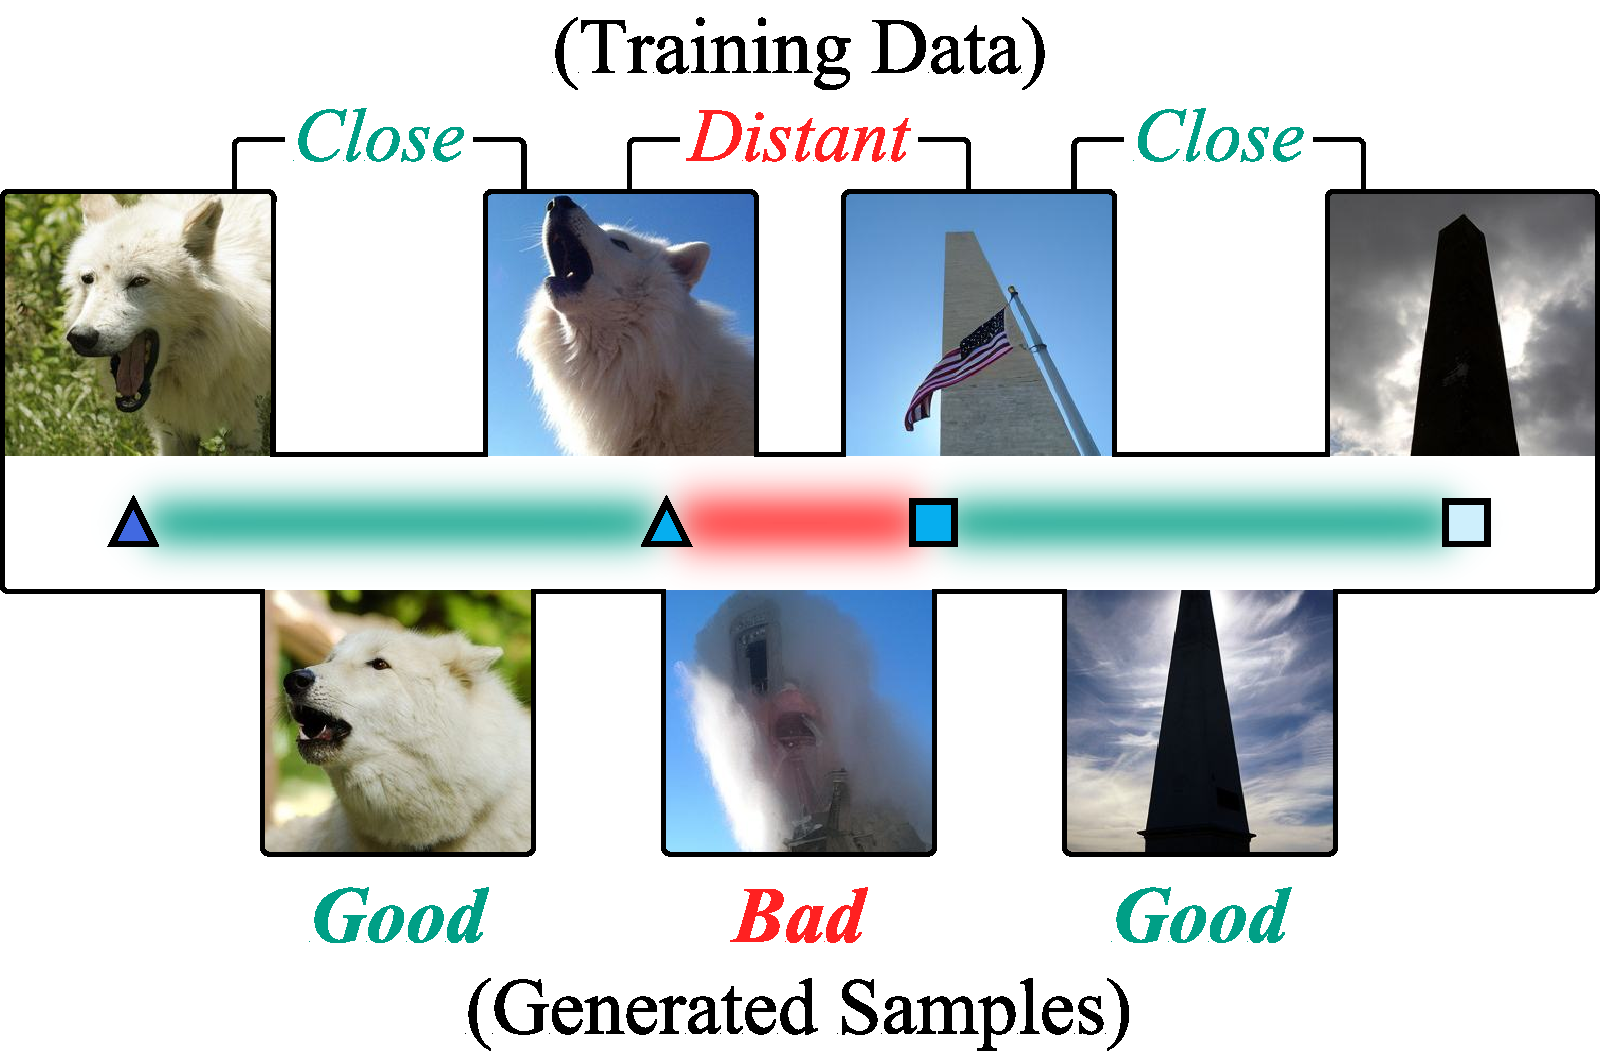
\includegraphics[width=0.5\textwidth]{figures/performance/good_generation_toy}
    \vskip -0.5\baselineskip
    \caption{\textbf{Comparison of \xred{``good''} vs.\ \xxgreen{``bad''} samples} on ImageNet, illustrated with an analogy to a 2D toy example. Toy training data: (\protect\tdA, \protect\tdB, \protect\tdC, \protect\tdD\!); generated samples: \protect\ellipseicon{xred}, \protect\ellipseicon{xxgreen}.}
    \label{fig:good-generation-toy}
\end{figure}